\section{Langkah-Langkah Percobaan}
\subsection{Crimping Kabel LAN}
\begin{enumerate}
    \item Siapkan kabel UTP, konektor RJ-45, crimping tool, dan LAN cable tester.
    \item Kupas bagian ujung kabel UTP sepanjang 2--3 cm menggunakan wire stripper untuk memperlihatkan inti kabel.
    \item Pisahkan dan luruskan tiap pasang kabel, kemudian susun berdasarkan standar warna (misalnya T568B).
    \item Potong ujung kabel agar rata sebelum dimasukkan ke dalam konektor RJ-45.
    \item Masukkan kabel yang sudah tersusun rapi ke dalam konektor hingga mencapai ujung.
    \item Gunakan crimping tool untuk menjepit konektor dan mengunci kabel di tempatnya.
    \item Uji kabel menggunakan LAN tester untuk memastikan setiap pin terhubung dengan benar.
\end{enumerate}

\subsection{Routing Statis}
\begin{enumerate}
    \item Buka aplikasi Winbox dan sambungkan router ke komputer menggunakan kabel LAN.
    \item Masuk ke router menggunakan MAC address atau IP default.
    \item Lakukan reset konfigurasi untuk memulai dari awal jika diperlukan.
    \item Atur IP address pada port \texttt{ether1} sebagai penghubung antar-router.
    \item Atur IP address pada port \texttt{ether2} sebagai jalur koneksi ke masing-masing PC.
    \item Tambahkan rute secara manual melalui menu \texttt{IP > Routes} dengan mengisi alamat tujuan dan gateway.
    \item Konfigurasikan IP, subnet mask, dan gateway secara manual pada laptop menggunakan pengaturan jaringan Windows.
    \item Lakukan pengujian konektivitas antar-laptop menggunakan perintah \texttt{ping}.
\end{enumerate}

\subsection{Routing Dinamis}
Rencana percobaan adalah mengatur routing dinamis menggunakan protokol seperti RIP atau OSPF. Namun karena routing statis belum berhasil, tahap ini tidak dapat dilanjutkan. Praktikum dihentikan pada tahap routing statis karena keterbatasan waktu dan kesalahan konfigurasi.

\section{Analisis Hasil Percobaan}
Pengkabelan LAN harus mengikuti susunan warna yang sudah ditentukan agar dapat berfungsi dengan baik. Jika terjadi kesalahan dalam menyusun kabel sebelum dipasang ke konektor, maka hasil pengujian menggunakan alat tester akan menunjukkan urutan lampu yang tidak sesuai standar. Dalam percobaan routing statis, konfigurasi tidak berhasil dilakukan, kemungkinan karena kesalahan dalam memasukkan alamat IP, baik pada router 1 dan router 2, maupun pada sambungan antara router dan laptop. Akibatnya, percobaan routing dinamis tidak dapat dilanjutkan karena tahap sebelumnya belum berhasil, ditambah dengan keterbatasan waktu yang tersedia.

\section{Hasil Tugas Modul}
\subsection{Berdasarkan tugas pendahuluan sebelumnya mengenai perancangan topologi jaringan dan tabel IP yang telah Anda buat, langkah selanjutnya adalah membuat simulasi jaringan menggunakan aplikasi Cisco Packet Tracer. Silakan lakukan konfigurasi pada masing-masing perangkat agar seluruh jaringan dapat saling terhubung dan berkomunikasi dengan baik.}
\begin{figure}[H]
    \centering
    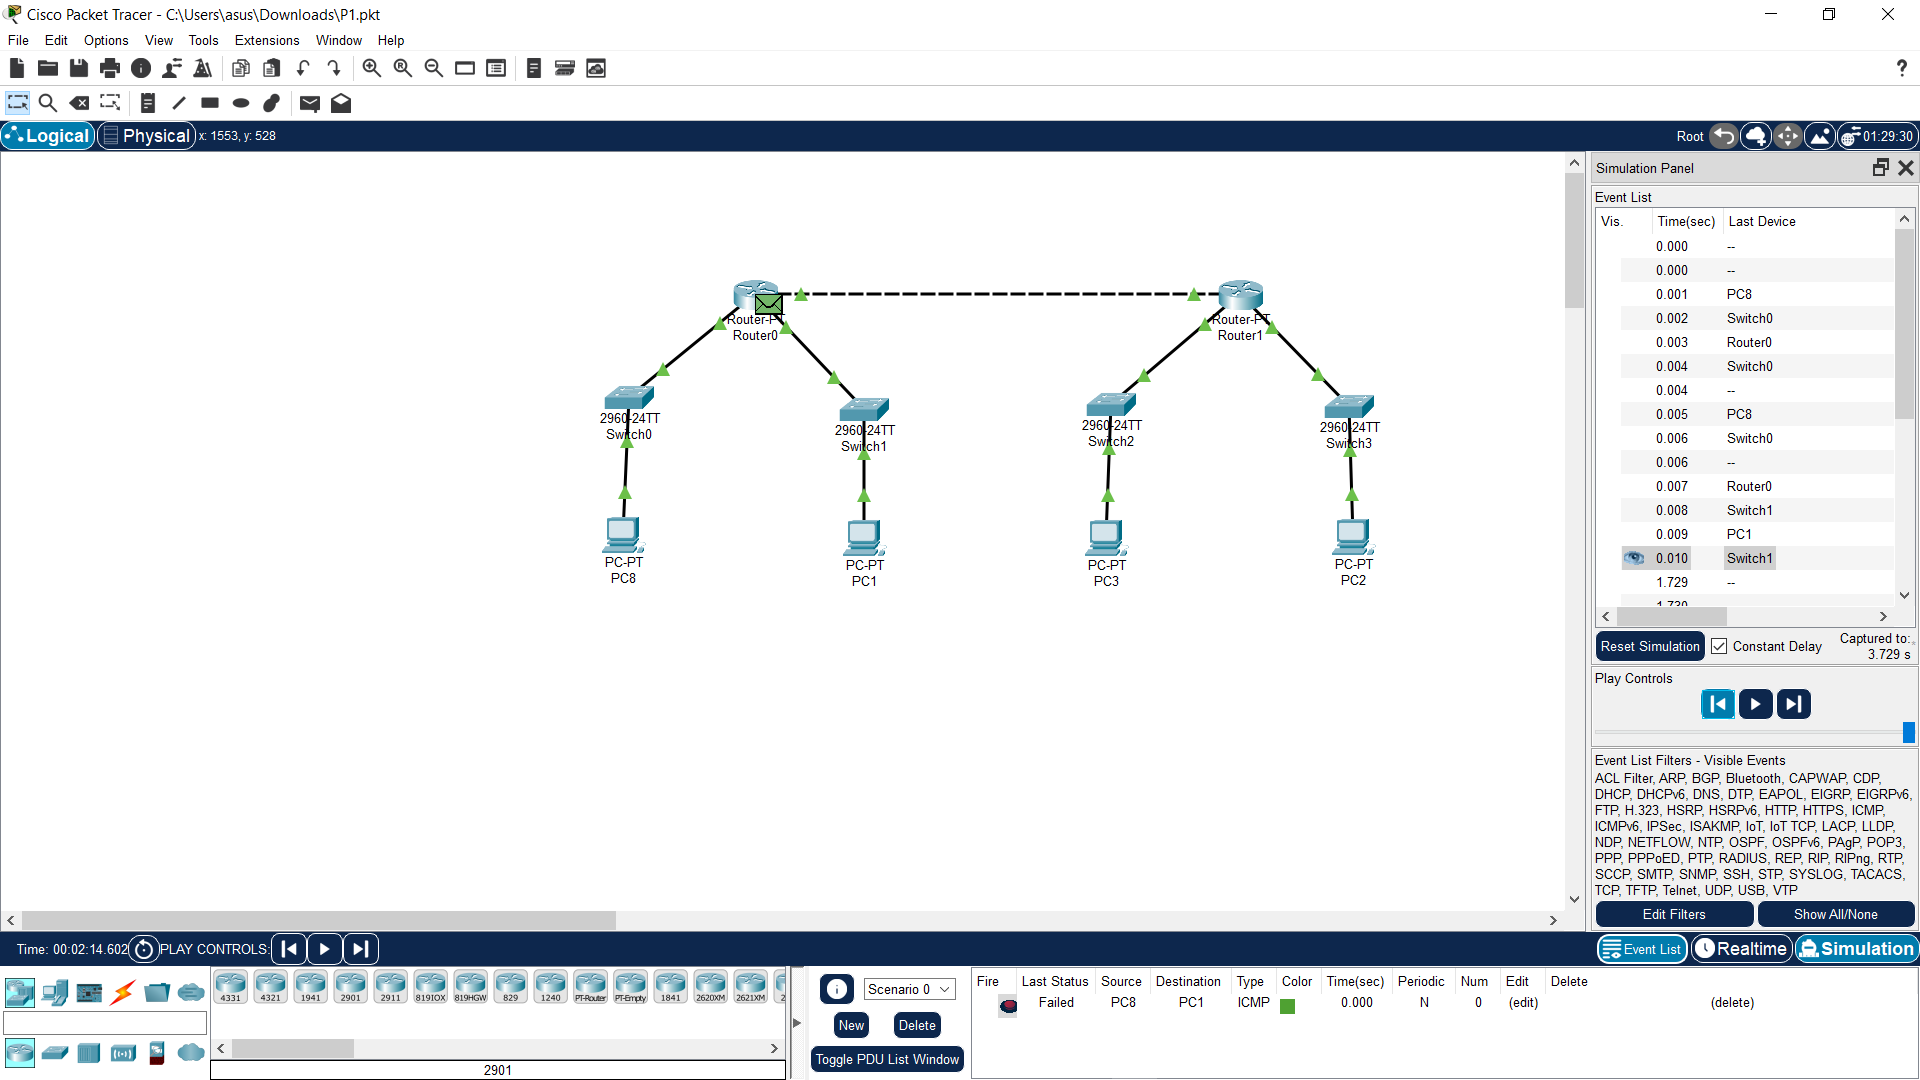
\includegraphics[width=0.8\textwidth]{P1/img/Paket.png}
    \caption{Topologi CISCO Packet Tracer}
    \label{fig:labelgambar}
\end{figure}

\subsection{Jelaskan apa kesulitan yang anda alami pada Praktikum.}
Selama praktikum, saya mengalami beberapa kendala yang cukup menghambat proses pelaksanaan. Kesulitan pertama terjadi saat proses pengupasan kabel, di mana saya tanpa sengaja mengupas terlalu dalam sehingga beberapa inti kabel terputus dan tidak dapat digunakan. Hal ini mengharuskan saya untuk mengulang dari awal dengan memotong kabel lagi. Selain itu, proses menyusun urutan kabel berdasarkan warna standar juga memerlukan ketelitian dan cukup memakan waktu, karena susunan yang salah akan menyebabkan kabel tidak berfungsi dengan baik. Kendala lainnya muncul saat mencoba melakukan uji konektivitas menggunakan perintah ping. Meskipun konfigurasi kabel LAN dan pengaturan di perangkat MikroTik sudah dilakukan sesuai prosedur, laptop tetap tidak dapat saling terhubung. Hal ini menunjukkan adanya masalah yang belum teridentifikasi pada konfigurasi jaringan atau perangkat yang digunakan. Dikarenakan hal tersebut dan waktu yang terbatas kelompok saya tidak dapat melakukan routing dinamis.

\section{Kesimpulan}
Berdasarkan hasil percobaan, dapat disimpulkan bahwa kabel LAN harus disusun sesuai dengan urutan warna standar agar dapat berfungsi secara optimal. Ketika dilakukan pengujian dengan alat tester, urutan lampu akan menunjukkan apakah susunan kabel sudah benar. Dalam praktik routing statis, kami mengalami kegagalan—kemungkinan disebabkan oleh kesalahan konfigurasi IP atau kendala pada perangkat yang digunakan, baik dari sisi perangkat lunak maupun perangkat keras. Akibat kegagalan ini, kami tidak dapat melanjutkan ke tahap routing dinamis.

\section{Lampiran}
\subsection{Dokumentasi saat praktikum}
\begin{figure}[H]
    \centering
    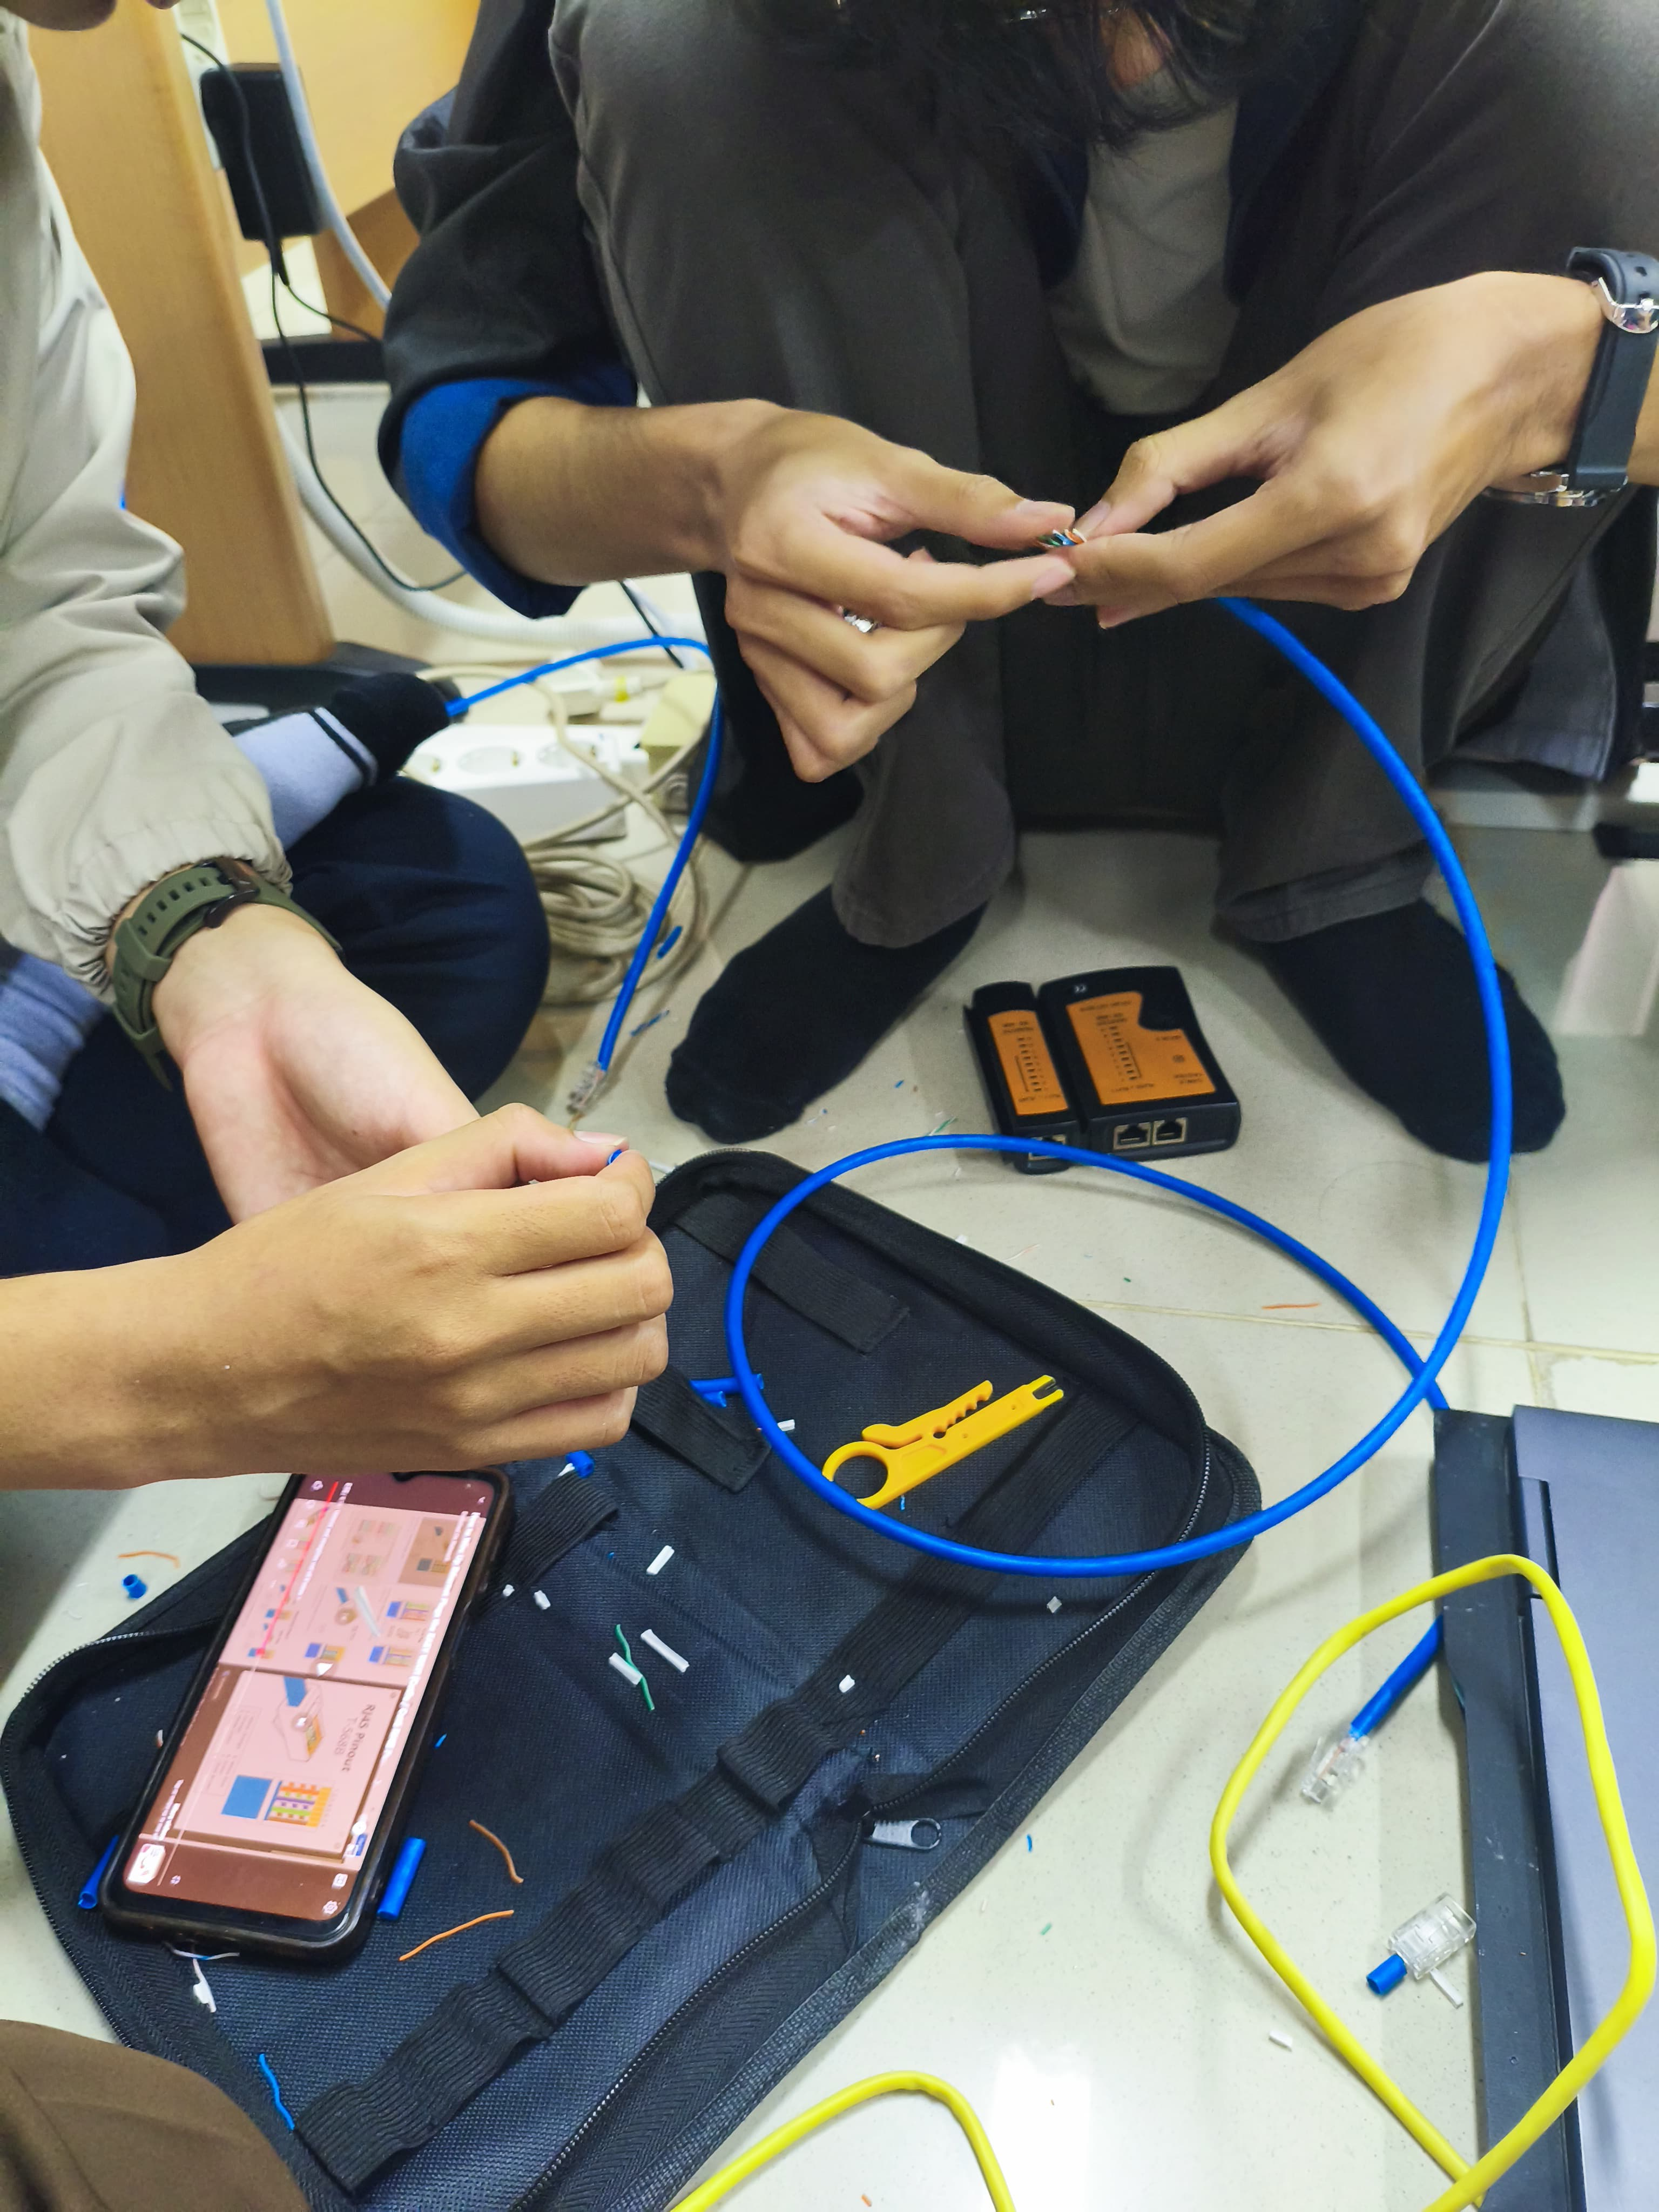
\includegraphics[width=0.5\textwidth]{P1/img/2.jpg}
    \caption{proses Crimping Kabel LAN}
    \label{fig:labelgambar}
\end{figure}
\begin{figure}[H]
    \centering
    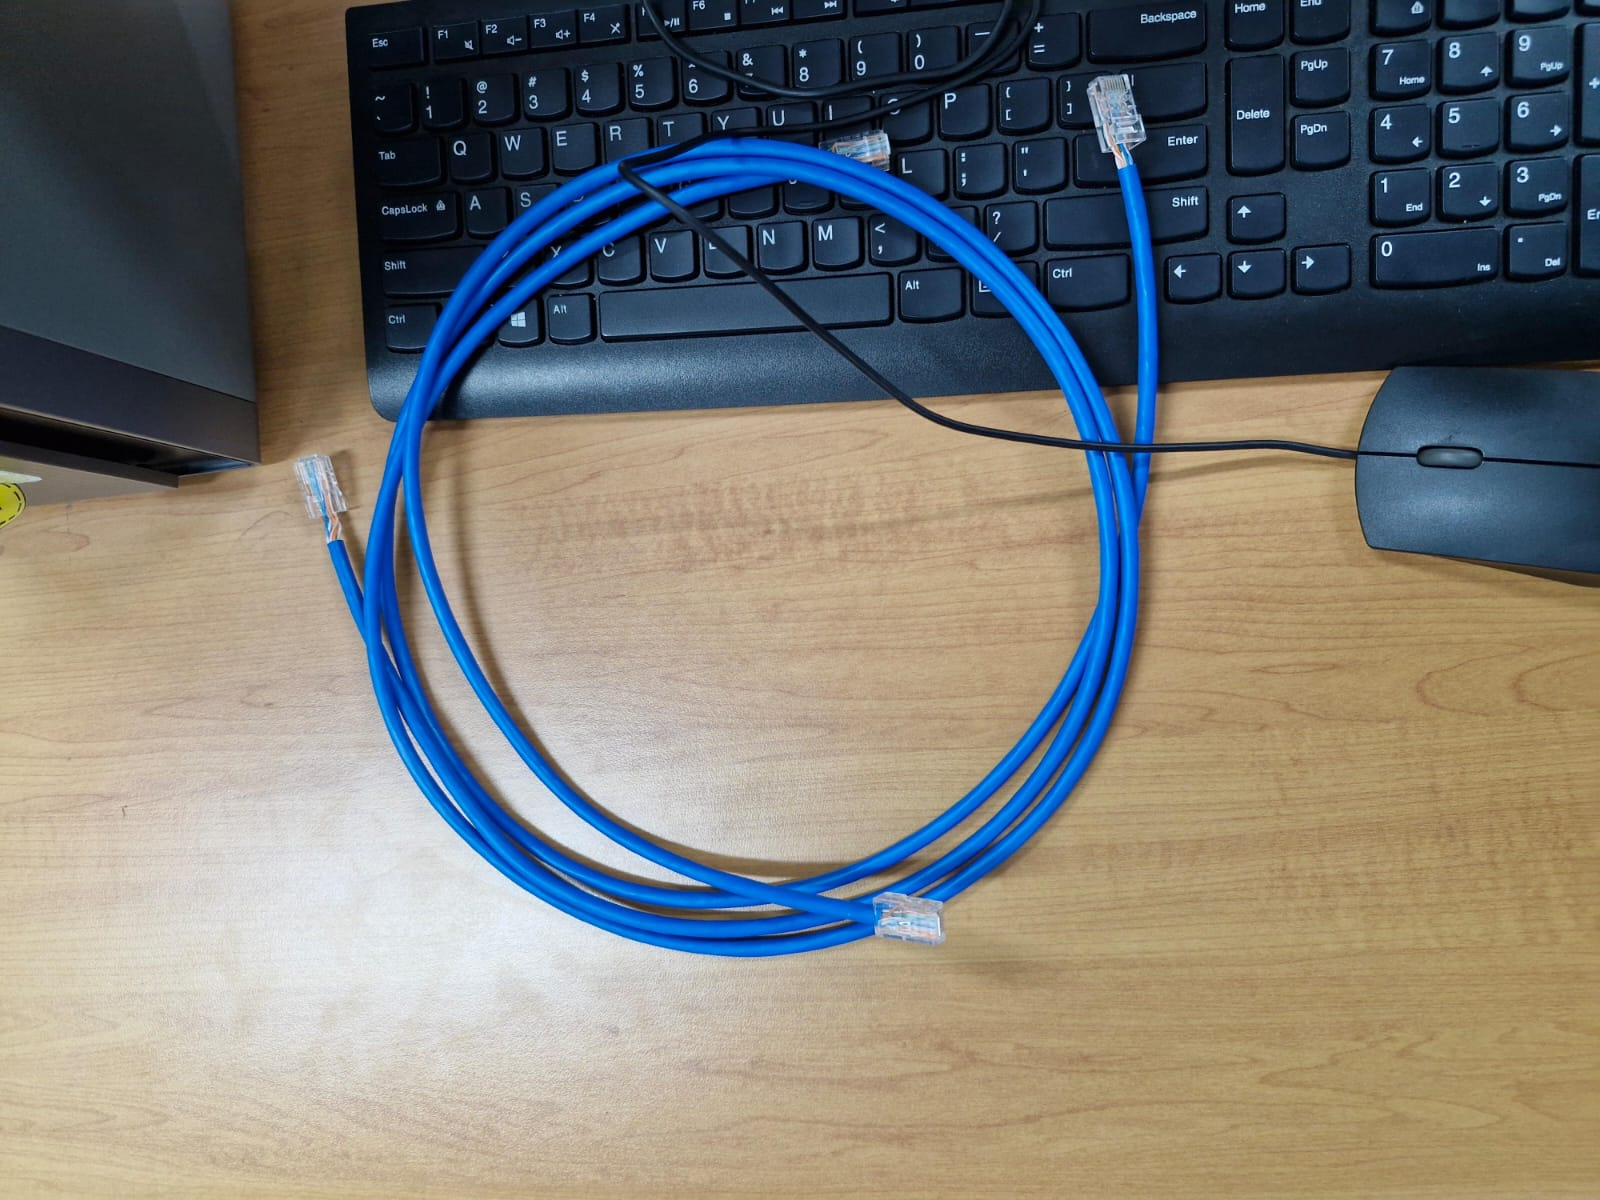
\includegraphics[width=0.5\textwidth]{P1/img/1.jpg}
    \caption{Hasil Crimping Kabel LAN}
    \label{fig:labelgambar}
\end{figure}
\begin{figure}[H]
    \centering
    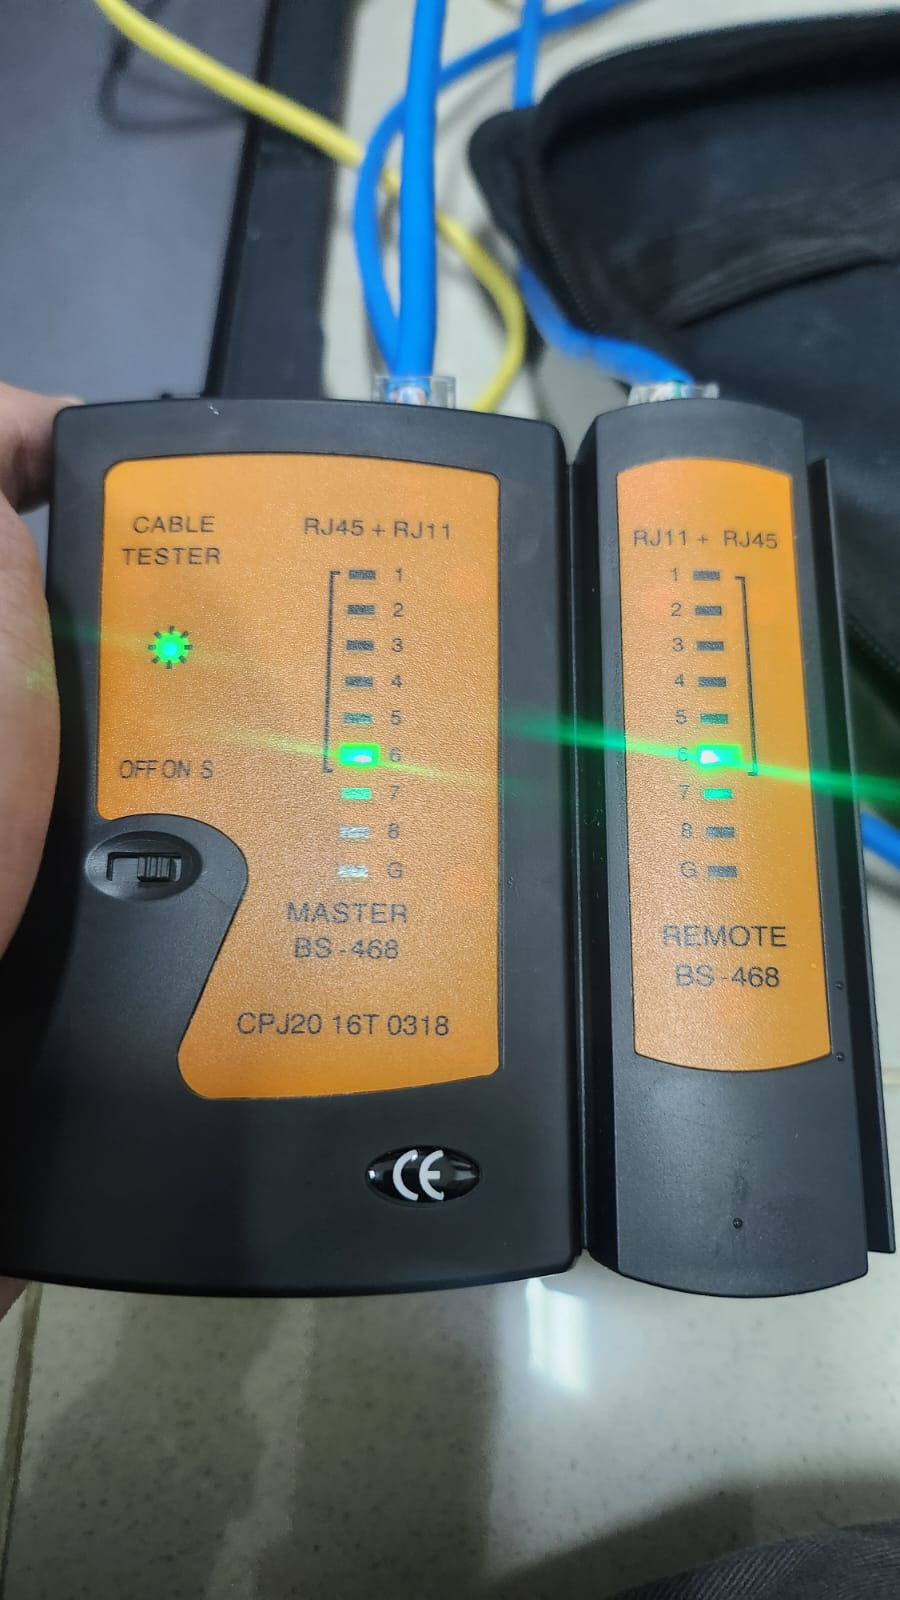
\includegraphics[width=0.5\textwidth]{P1/img/3.jpg}
    \caption{Testing Kabel LAN}
    \label{fig:labelgambar}
\end{figure}
\begin{figure}[H]
    \centering
    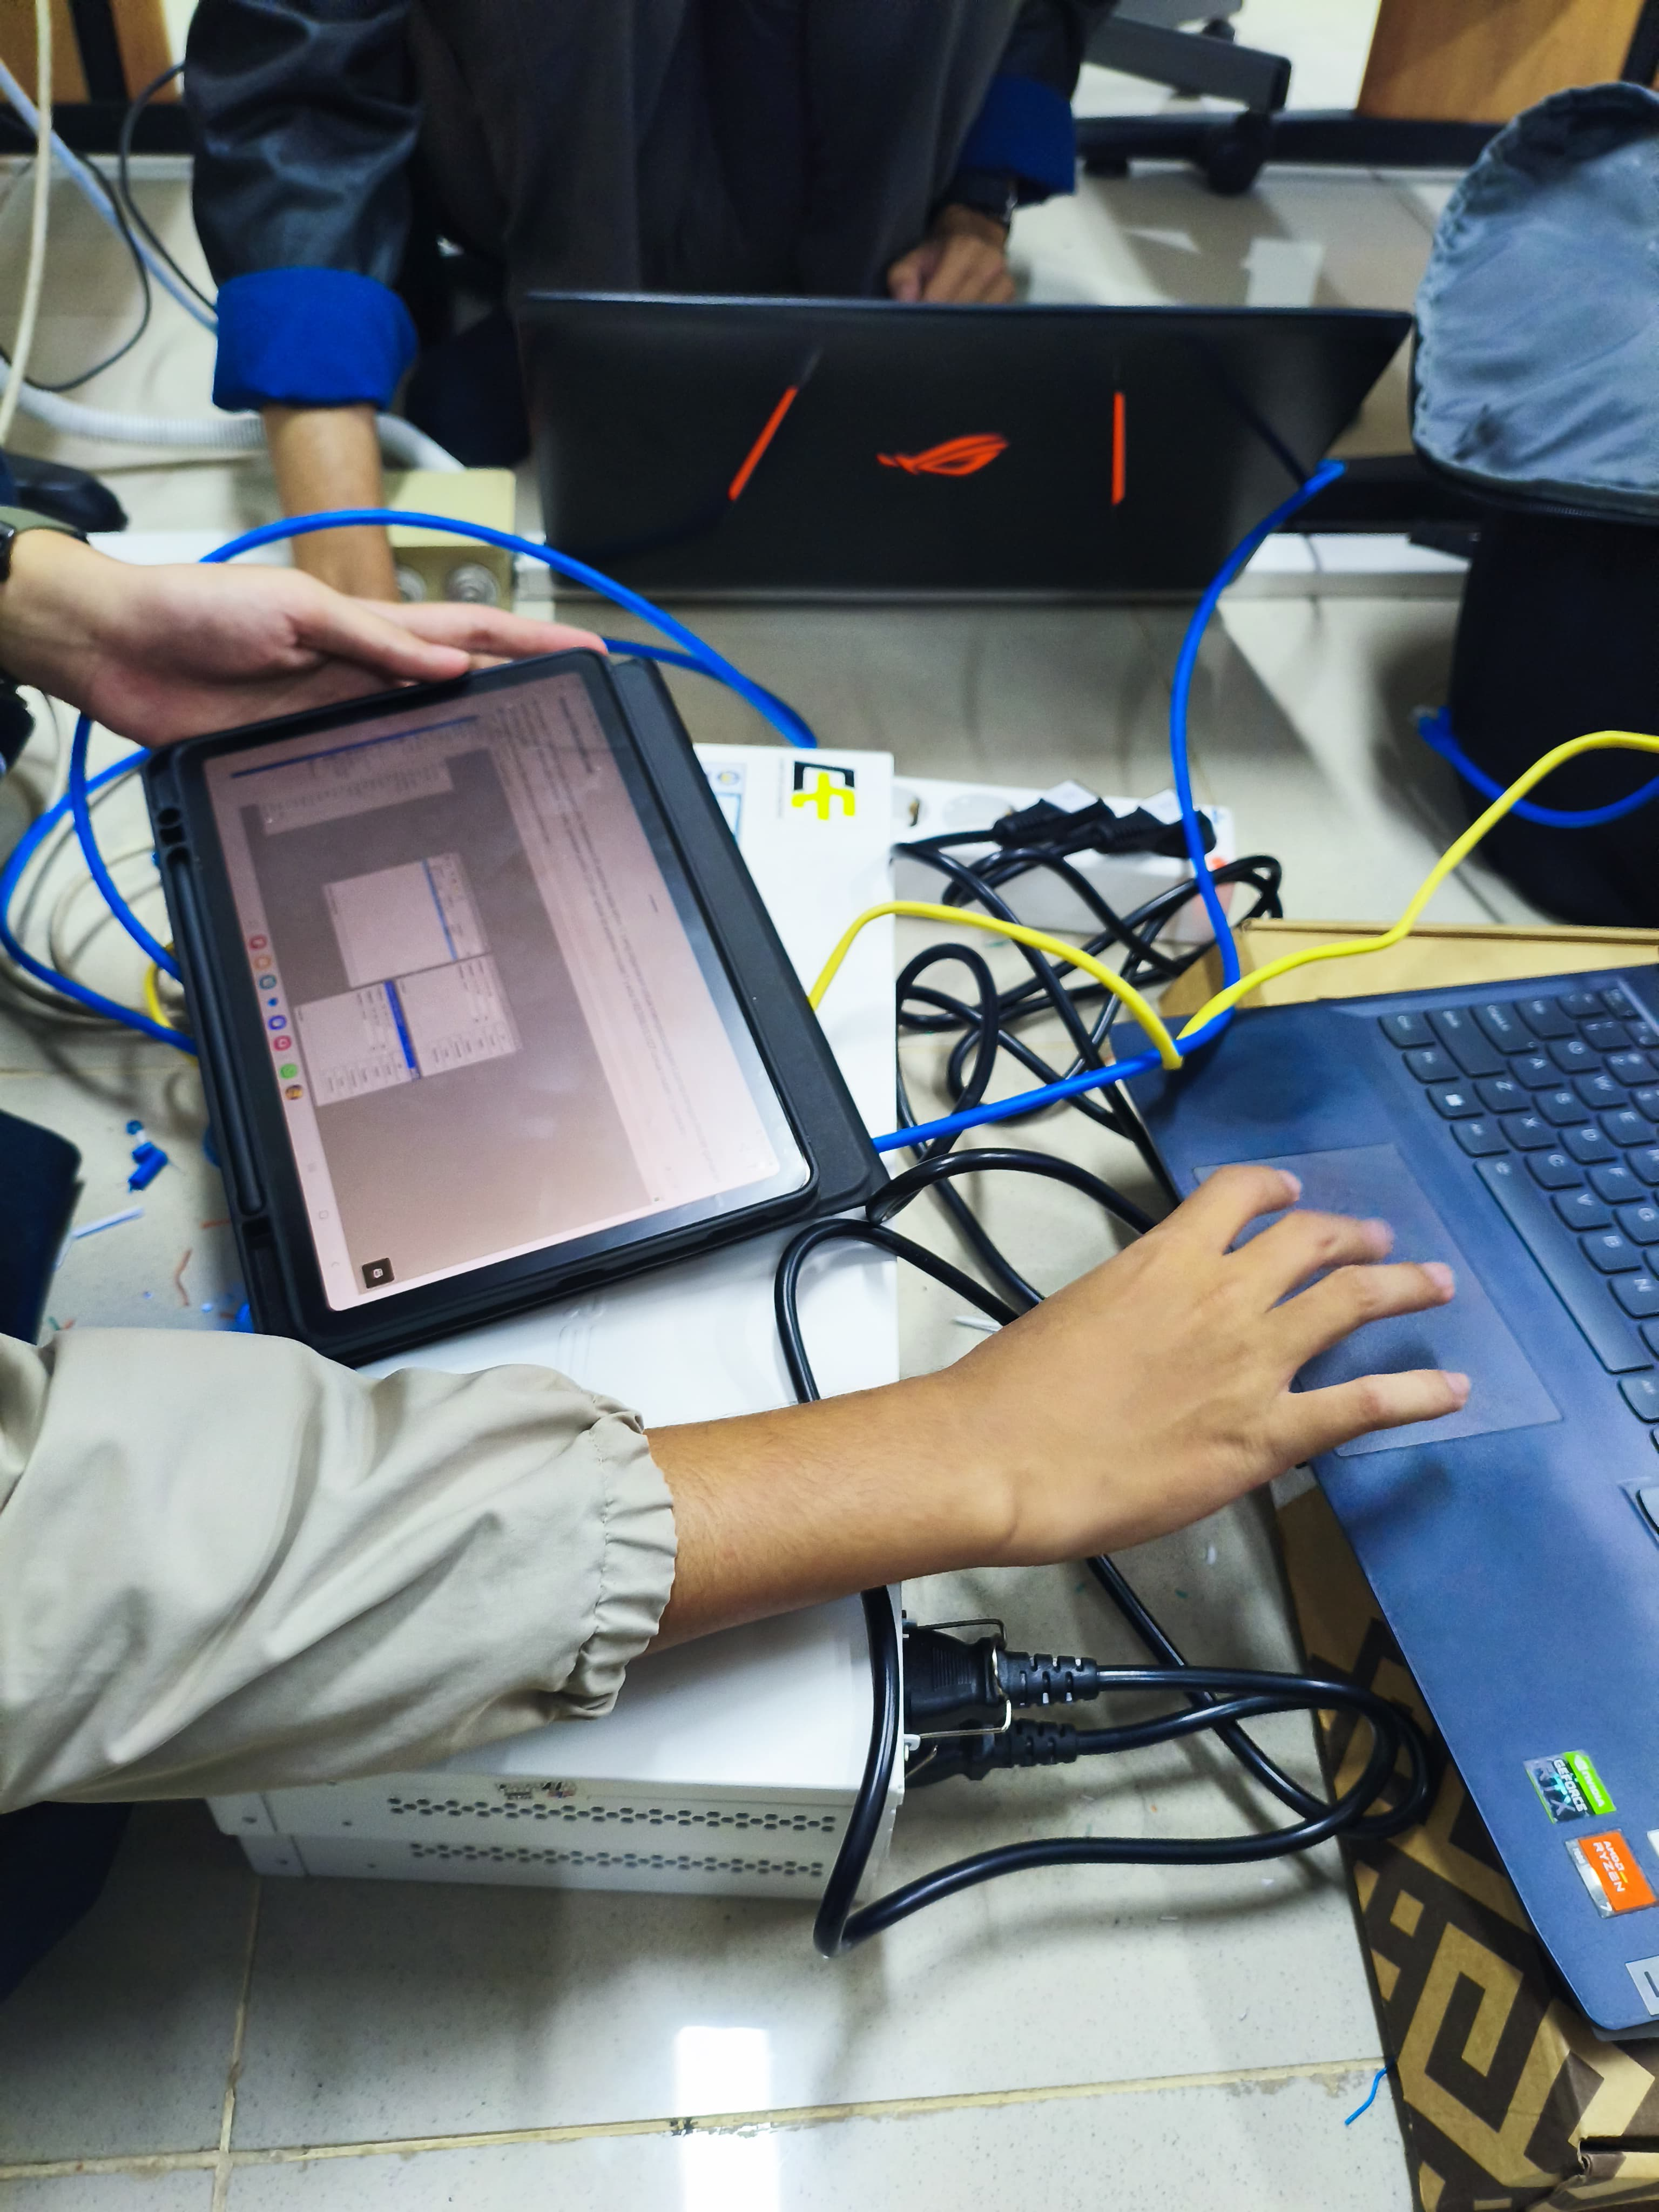
\includegraphics[width=0.5\textwidth]{P1/img/5.jpg}
    \caption{Memasukkan Data-Data Ke WinBox}
    \label{fig:labelgambar}
\end{figure}
\begin{figure}[H]
    \centering
    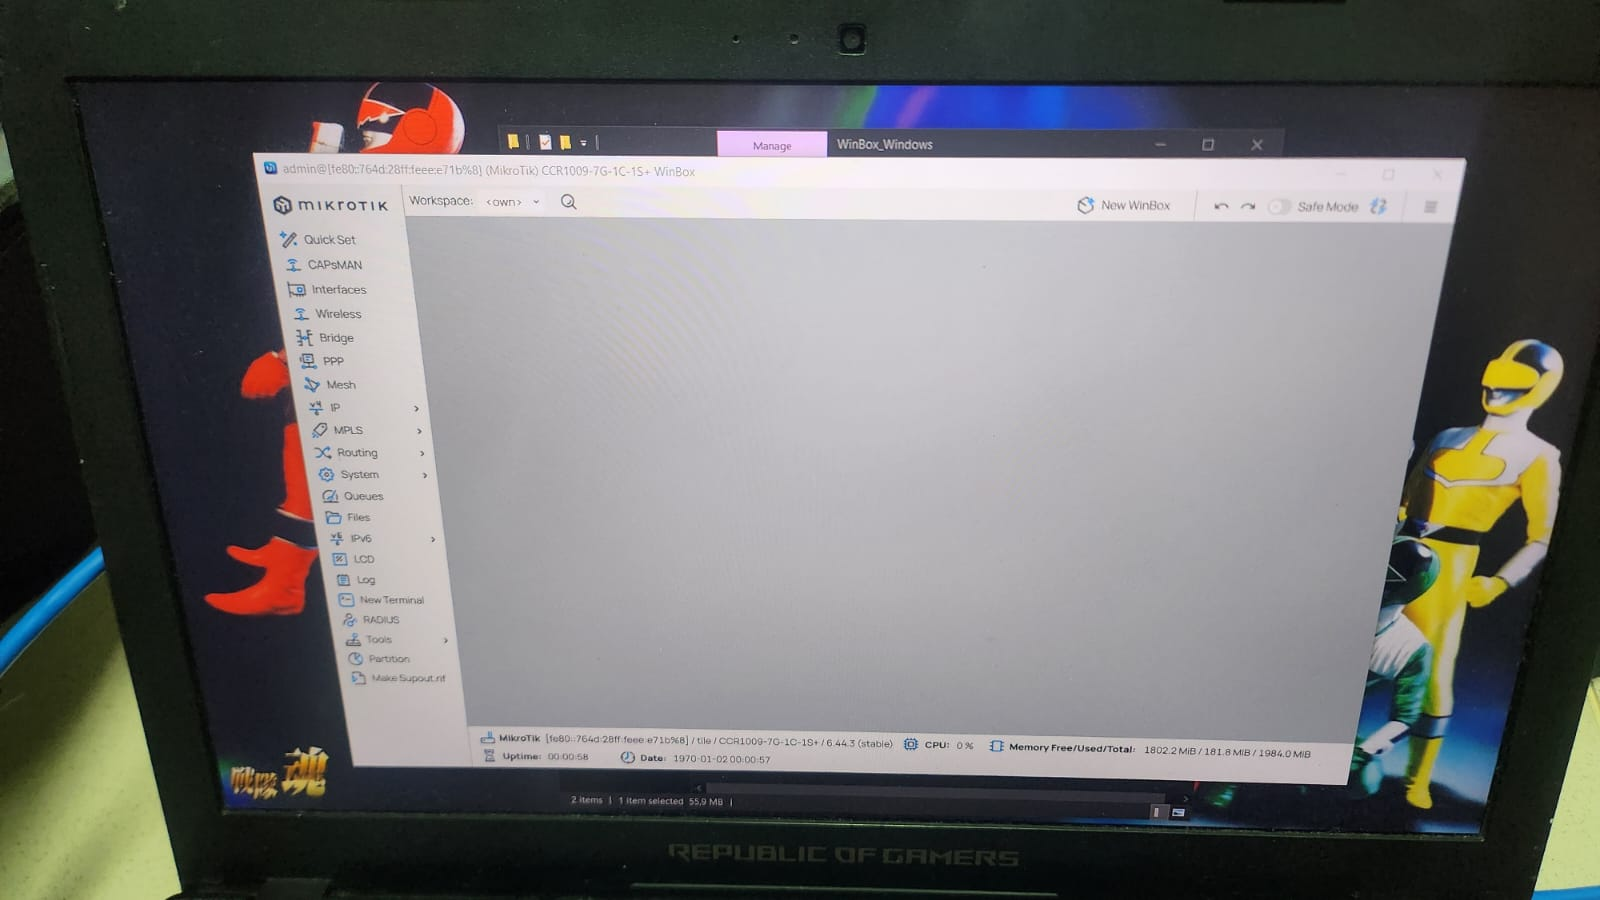
\includegraphics[width=0.5\textwidth]{P1/img/4.jpg}
    \caption{Resetting Router di WinBox}
    \label{fig:labelgambar}
\end{figure}
\begin{figure}[H]
    \centering
    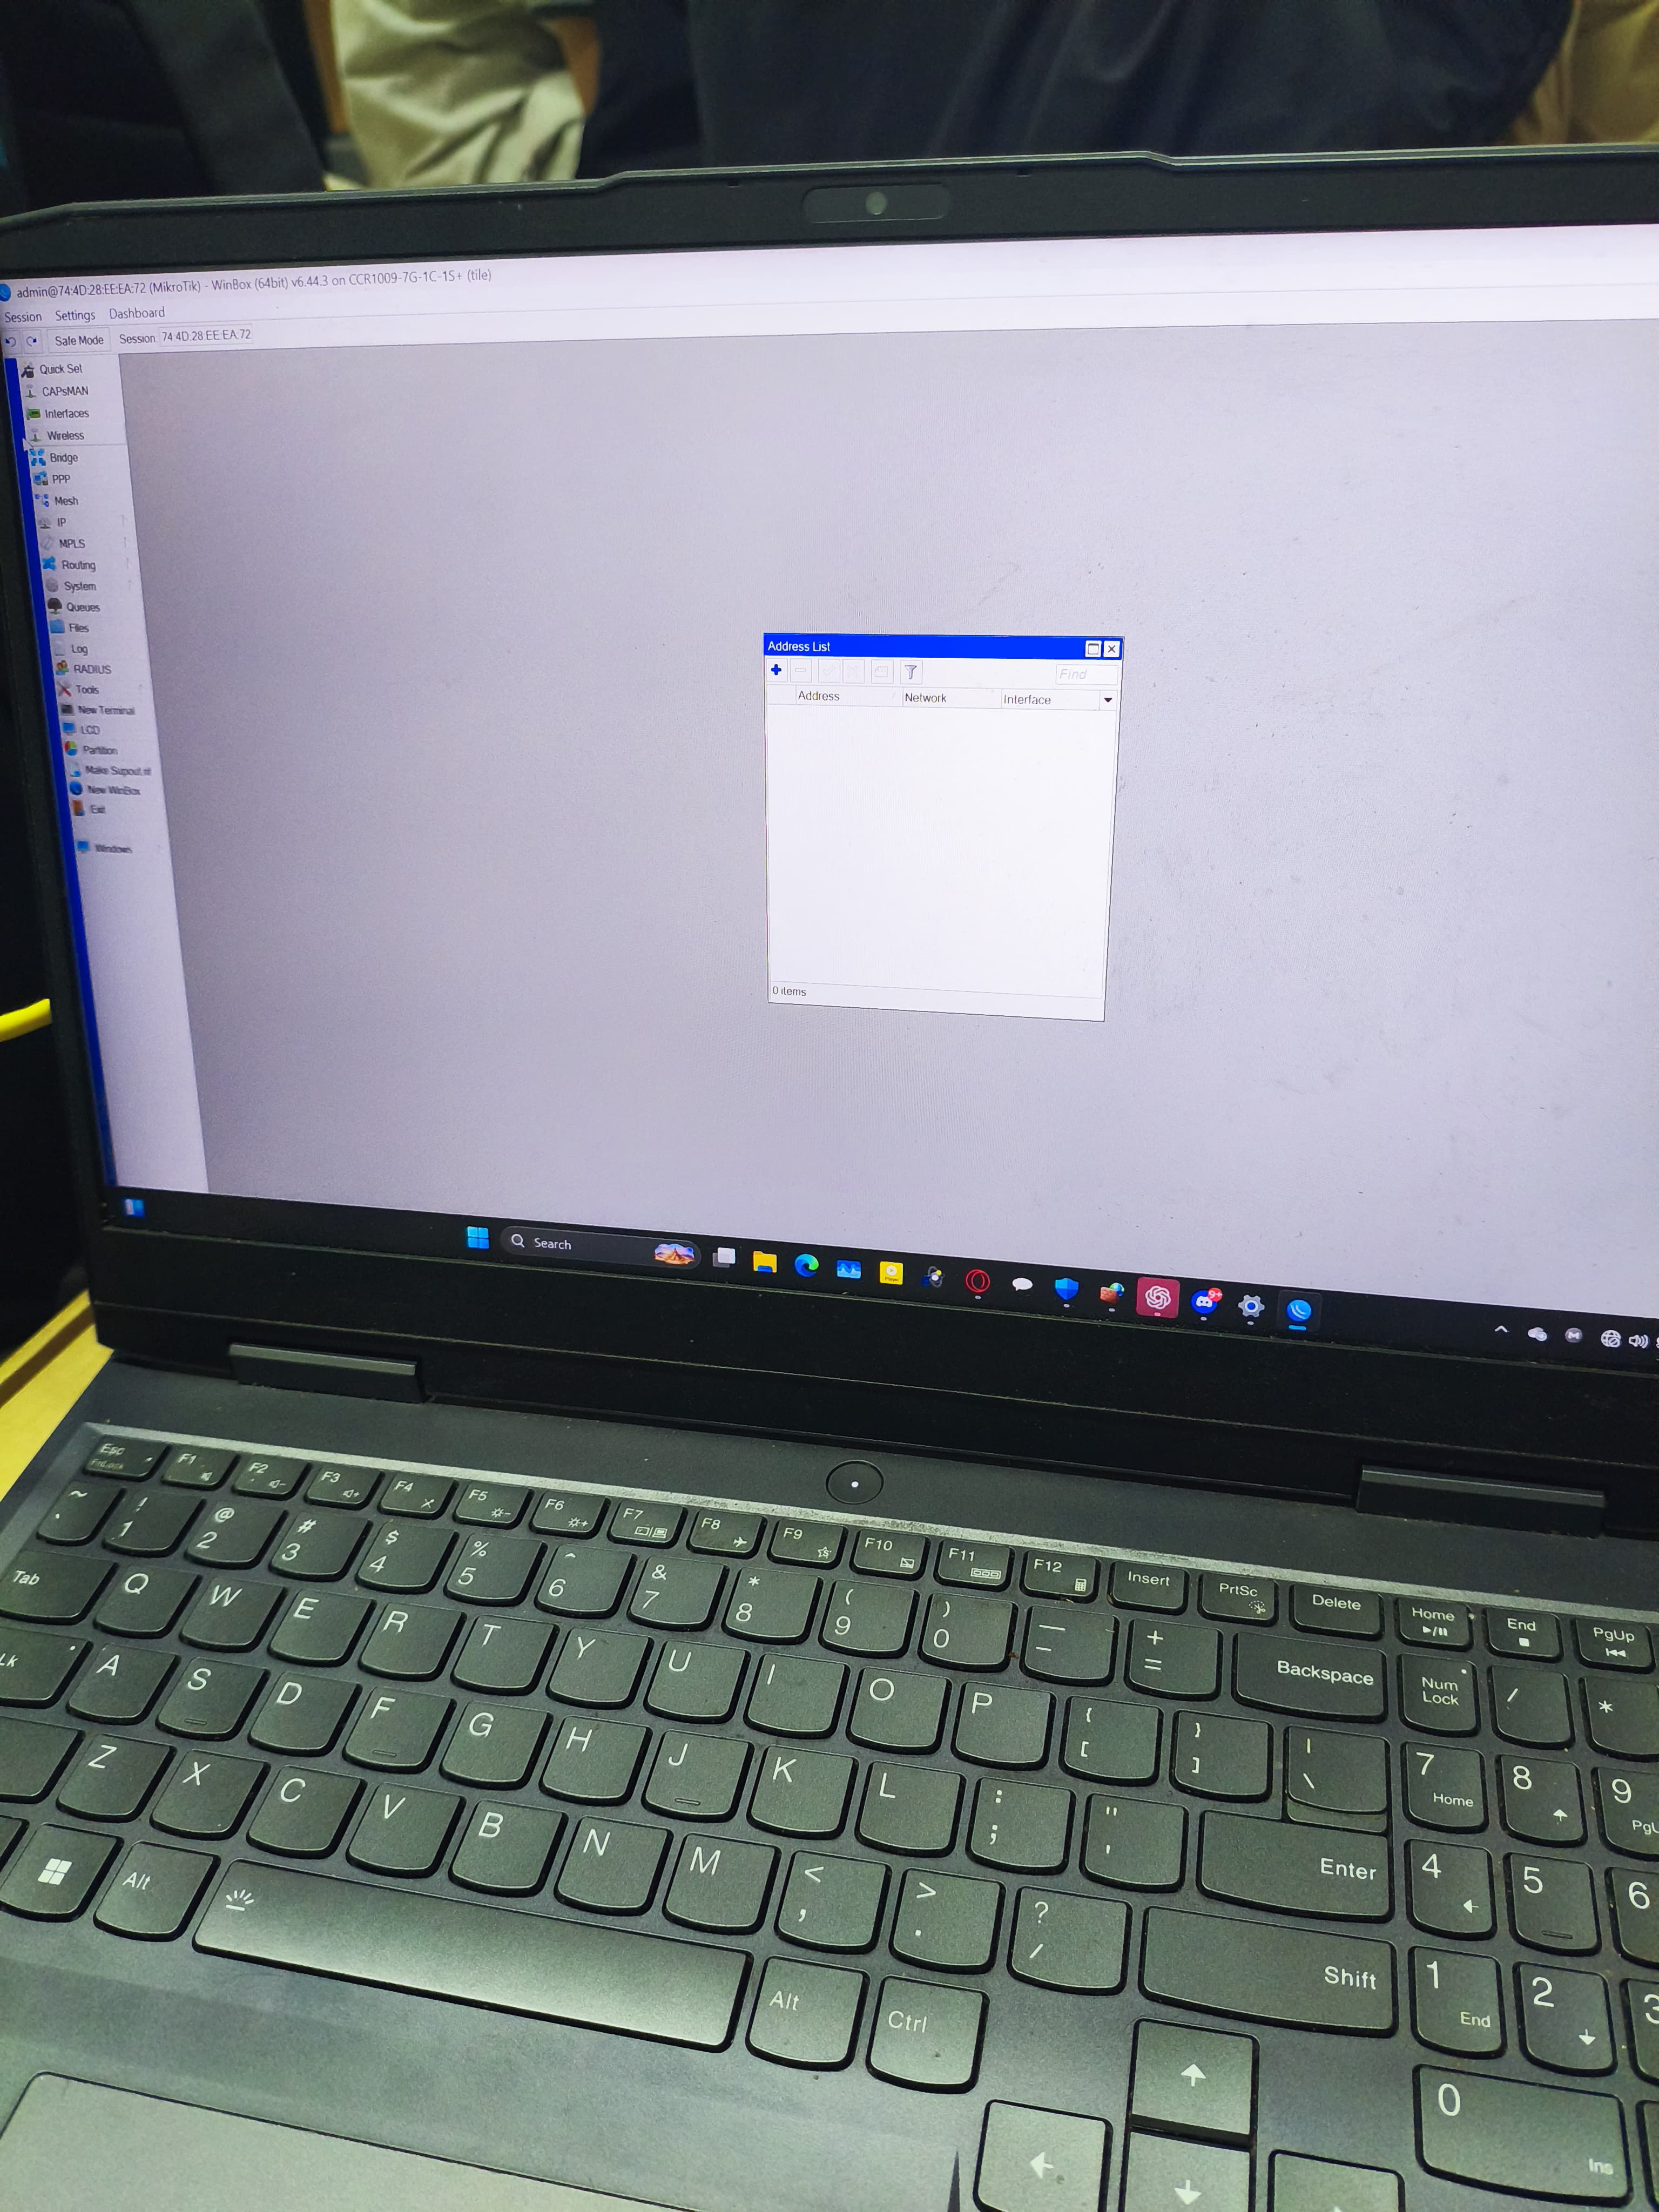
\includegraphics[width=0.5\textwidth]{P1/img/6.jpg}
    \caption{Tampilan WinBox}
    \label{fig:labelgambar}
\end{figure}
\begin{figure}[H]
    \centering
    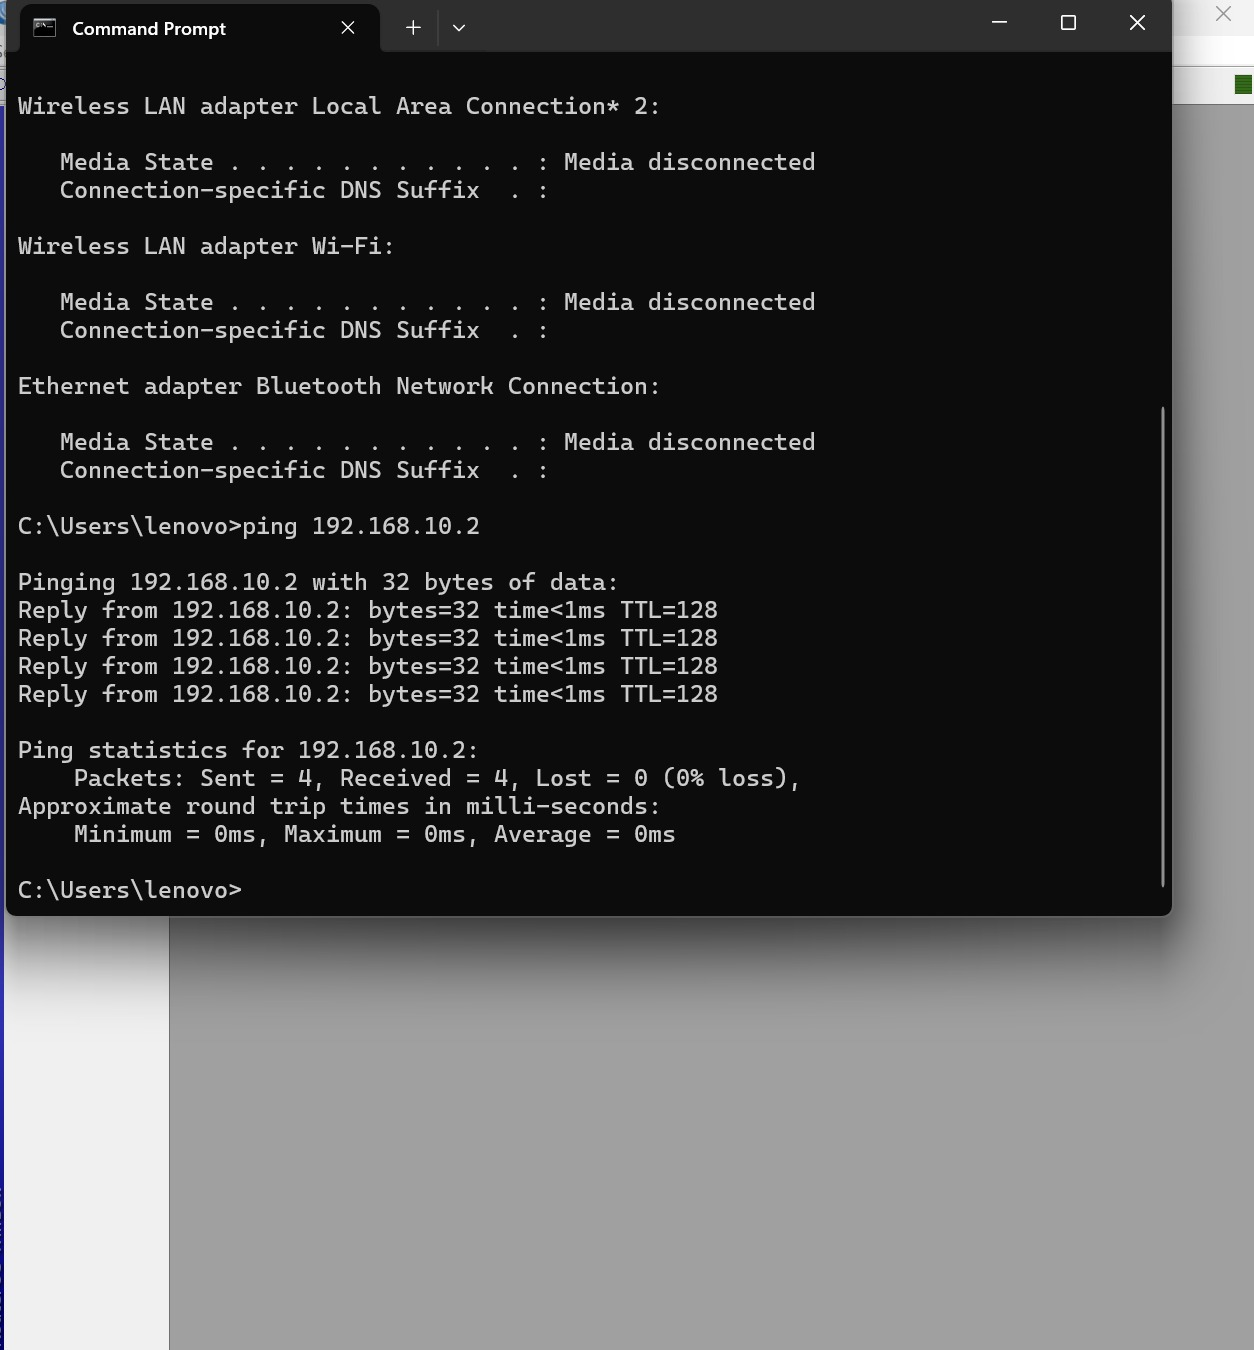
\includegraphics[width=0.5\textwidth]{P1/img/8.jpg}
    \caption{Hasil PING Laptop 1}
    \label{fig:labelgambar}
\end{figure}
\begin{figure}[H]
    \centering
    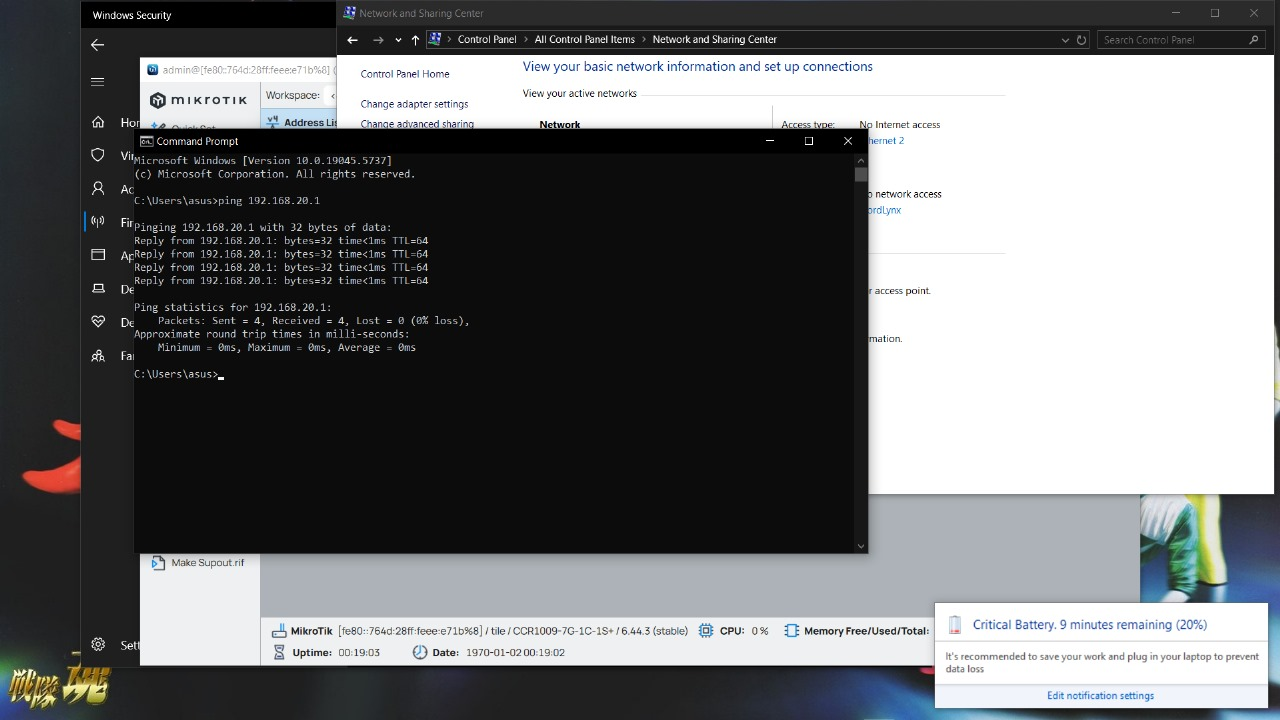
\includegraphics[width=0.5\textwidth]{P1/img/7.jpg}
    \caption{Hasil PING Laptop 2}
    \label{fig:labelgambar}
\end{figure}